
\section{Introduction and Problem Statement}

%XXX general idea. maybe introduce introduce a table of abbreviations?

% (Give a brief overview of App Store ecosystem and intermediaries.) 

% (Explaining the problem for each of the 3 main flows. Problem of double attribution, problem of refutation,....)

App stores are a distribution channel between the developer and the end user. Although software distribution exists since there is software development, the current model of smartphone became popular with the launch of Apple App Store in July 2008, and with its pre-load in iPhone 3G.

In the same year, but later in August 2008, Google announced the launch of Android Market\cite{wiki:market}, the App Store for Android.

These initial app stores followed a centralized model where one entity is responsible for assuring the core features of software distribution: file delivery, app discovery, financial transactions, and app approval. As the smartphone userbase grew, the centralized model started to show severe flaws. The flaws and problems identified are strongly related with the existent model: lack of trust and economical efficiency. 

By not being transparent, app stores don't earn the trust among the different stakeholders: developers, advertisers, users, and OEM manufacturers. Being centralized, they cannot benefit of a shared and crowdsourcing economy. Being closed source and hiding data, they don't promote competition and innovation.

% XXX not transparent: how?
% XXX hiding data: what data?

The App Coins protocol covers three core app store use cases:

\begin{itemize}
\item {\bf Advertising inside the app store}: the transactional flow where a developer pays for a user to install his app or game. There are different advertising models depending on the action that triggers the actual payment of the Ad: CPI (Cost per Installation), CPA (Cost per Action), CPM (Cost per thousand impressions),... There are different technology and platforms to support it: Ad networks, Exchanges and RTB (Real Time Bidding).
\item {\bf In-App Purchase}: when there is something that the user wants to buy inside the app or the game, like gems or unlock levels, the purchase mechanism is done through the app store. To enable those transactions the developer has to integrate the SDK from the App Store or to use the App Store API.
\item {\bf App approval}: in order for the app to be available the developer has to go through an approval process where the App Store screens the app through automatic tools like anti-virus, anti-malware tools, and static and dynamic code analysis platforms and then manually tests it.
\end{itemize}


\begin{figure}[!ht]
\centering
%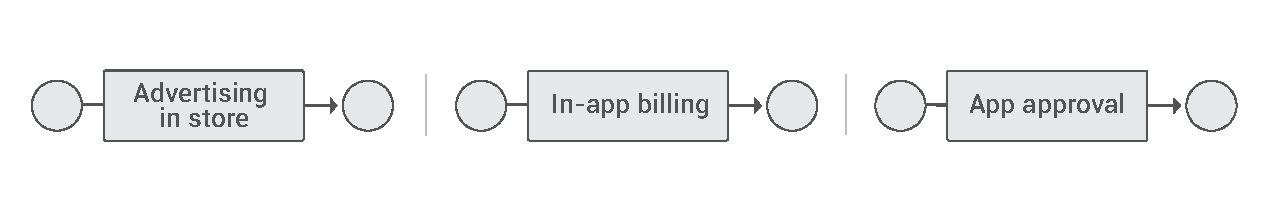
\includegraphics[width=11cm]{diagrams/current_flows.eps}
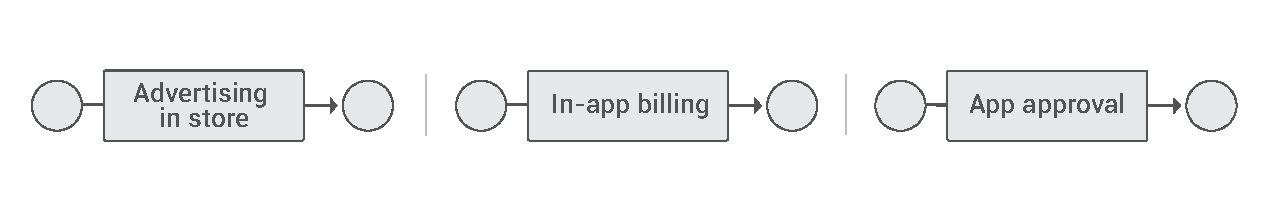
\includegraphics[width=\textwidth]{diagrams/current_flows.eps}
\caption{Individual existent core flows in app stores.}
\label{fig:exist_flows}
\end{figure}




In the next sub-sections, we'll analyse each of the above flows and the main problems faced today.

\subsection{Advertising}


Currently, the three flows presented in figure \ref{fig:exist_flows} don't have any interaction among them. They are isolated and handled by different App Store teams. The resources and information generated by one flow are not reused by the others. The intermediaries are many and were introduced to solve the lack of trust and the need to integrate with different players in a fragmented market.  

% XXX which flows: the flows cannot be easily identified
% XXX The resources ... sentence seems to be redundant.


In the next sub-sections, we'll analyse each of the above flows individually and the main problems faced today.


For a developer or a publisher, the most natural place to advertise an application or game is where the users are looking for that kind of content: the app store.

\begin{figure}[!ht]
\centering
%\includegraphics[width=11cm]{diagrams/current_flows.png}
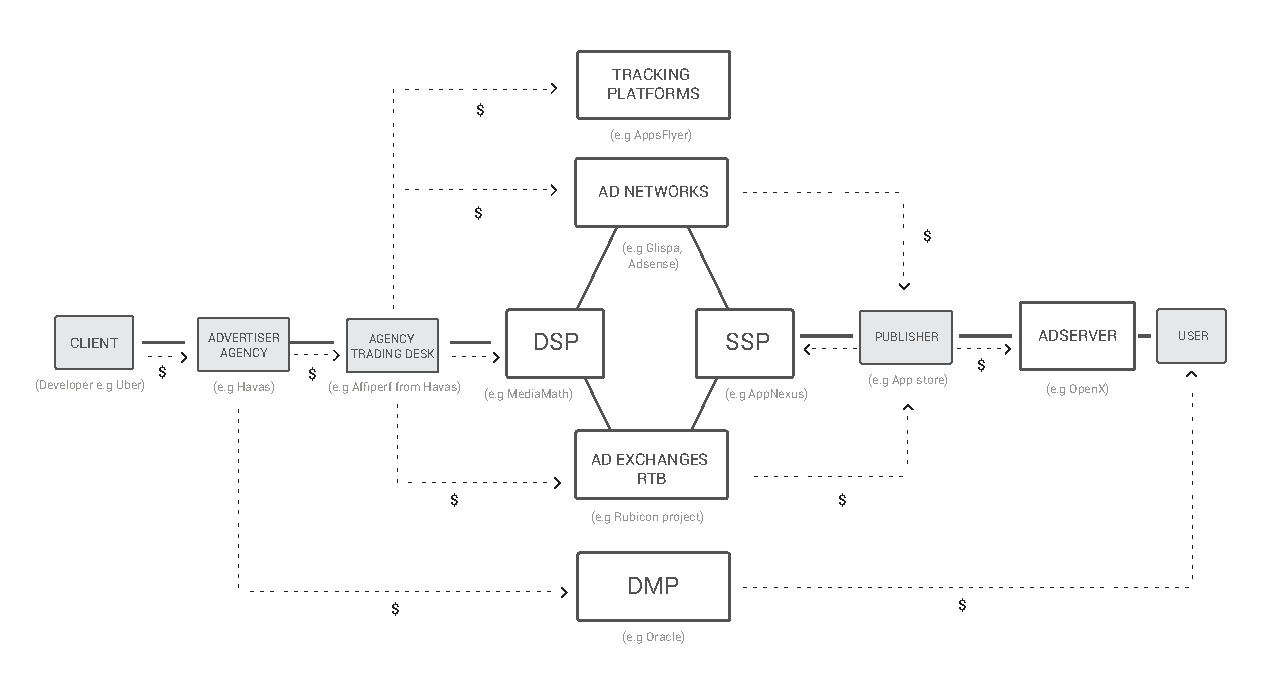
\includegraphics[width=\textwidth]{diagrams/cpi_flow.eps}
\caption{Cost per Installation (CPI) ecosystem.}
\label{fig:exist_flows}
\end{figure}

For simplicity, we will focus in the Cost per Install (CPI) model, since the difference to the other models, like Cost per Action (CPA) or Cost per thousand impressions (CPM), is a matter of who shares the risk and captures the value.

In an advertising model where the advertiser (developer) bids for an installation, we have the three different moments:


\begin{itemize}
\item {\em Campaign creation}: the developer (advertiser) defines the conditions for the ad to run in the store. Typically, he establishes a value for the bid representing the value that is willing to pay for an install. There are other types of conditions called ``filters'' and representing target requirements: it must run in a specific country, a specific smartphone, a specific operating system version,...
\item {\em Impression}: when the campaign conditions are met and the bid is competitive, the ad is shown. The user may click in the ad to see the complete description of the App.
\item {\em Install}: if the user installs the App, thus converting the impression, an attribution is due and the corresponding money is transferred.
\end{itemize}

% Create a itemize list above 

At each of the above moments, the lack of trust between the developer and the user carries different risks. Table \ref{tab:risks} summarizes the different risks at each stage.

% table

\begin{table}[ht]
\centering
\begin{tabular}{|l||l|l|l|} \hline
{\bf Role} & {\bf Campaign} & {\bf Impression}  & {\bf Install} \\ \hline
{\bf User} & & & Is not a real user \\ 
 & & & ({\em R1:Risk of fake person}) \\ 
 & & & Double conversion  \\
 & & & ({\em R2:Risk of double attribution}) \\
 & & & Don't use the app  \\
 & & & ({\em R3:Risk of no attention}) \\  \hline
{\bf Publisher  /}  & & & Selling the data to third-parties \\ 
{\bf App store} & & & ({\em R4:Risk of data leak})\\ \hline
{\bf Developer} & Not enough funds & Run out of & Don't pay \\  
 & to start campaign & budget & the conversion \\  
  & ({\em R5:Risk of default}) & ({\em R5:Risk of default}) & ({\em R6:Risk of repudiation}) \\  
\hline\end{tabular}
\caption{Risks in advertising industry classified by action and by role.}
\label{tab:risks}
\end{table}

The risks presented above are today managed in different ways by the advertising ecosystem and have different impacts:

\begin{tcolorbox}[enhanced jigsaw,sharp corners, drop fuzzy shadow=ShadowColor]

The {\bf\em R1.2:Risk of fake person} consists of the impression of the ad and later installation being presented to a non-real person (bot,...) with the purpose of deluding the advertiser. 


The {\bf\em R1.2: Risk of double attribution} happens with the possibility of the same user to count twice as a conversion, leading the developer to pay two times what was due.


The {\bf\em R1.3:Risk of no attention}  consists in the user install the app that is being advertised but not paying any attention to it. He may or not open the app, but not interact with the app, leading to a zero return-of-investment.


The {\bf\em R1.4:Risk of data leak} consists in the information regarding the user being leaked to third-parties for advertising purposes. Information about the user preferences is aggregated in Data Management Platform (DMP) platforms and later used by advertising in programmatic / RTB targeting. 

The {\bf\em R1.5:Risk of default} consists in the developer creating a campaign but not having enough funds to pay the conversions that are generated in that campaign. Therefore not paying the due amount.


The {\bf\em R1.6:Risk of repudiation} happens when the developer doesn't recognize the installation, failing to attribute the conversion to the publisher. The attibution is generally monitored by tracking platforms like AppsFlyer, Adjust or Kochava that have multiple variables that can be changed by the developer to define what it considers a real attribution. These variables can take in account the time window period between the click URL and the conversion, the network fingerprint, amoing others. Attribution, or the lack of attribution, is mining the industry with only 15\% to 25\% of the real installations being considered conversions.

%XXX what does mining the industry mean?
%XXX provide reference for the 15-25% statement

\end{tcolorbox}

These risks in the Advertising flow will be considered in a section ahead in the design of the AppCoins blockchain.


\subsection{In-App Billing}

% Description of In-App Billing inside the stores

In-App Billing (IAB), also called In-App Purchase, consists in the possibility for the user to buy digital items inside an app or a game. Although those items are perceived to be bough inside the App, the items are bought through the app store.

\begin{figure}[!ht]
\centering
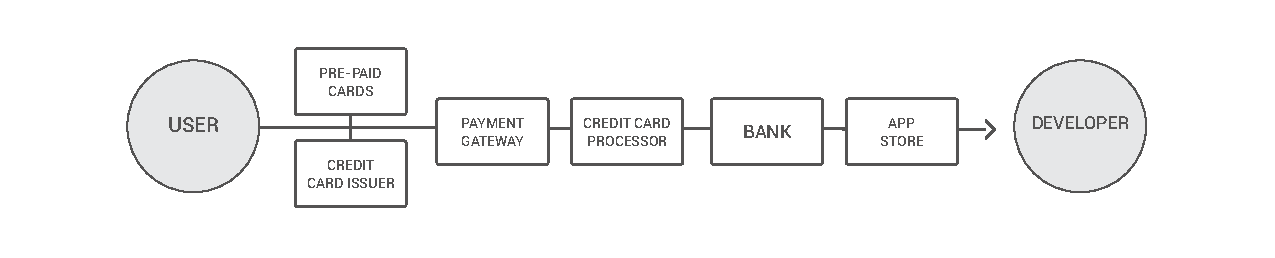
\includegraphics[width=\textwidth]{diagrams/iab_flow.eps}
\caption{Current IAB flow and intermediaries.}
\label{fig:iab_flow}
\end{figure}


The need for the transactions for go through the app store were introduced as mandatory by Apple App Store and then by Google Play. The conditions for the developer's App to be distributed is that all the financial transactions have to be managed by the app store. 

The app store adds some value to this flow: 1) it may know the customer already and have is payments data thus easing the entrance hurdles for the user and providing a better user experience, 2) has the trust of the user where the developer may have not 3) develop the technology necessary, allowing the developer to focus in the app development.

Although IAB represents a market with a huge volume of transactions processed by Google Play and Apple, there is still two big challenges.

%XXX provide source for "huge volume of transactions by ..."

The number of users with a credit card loaded in the store is still a minority. Only small part of the world population has access to credit card. Alternative methods like pre-paid cards are an approach but they are physical and depend of points of sale, therefore don't scale well.

On the other hand, some of other payment methods like carrier billing have prohibitive margins that compromise the revenue share of 70\% for the developer. In some markets, the margin of the telecom operator varies between from 35\% to 60\% of the cost of the transaction. The reasons given by the telecom operators are: 1) high risk of fraud that has to be compensated 2) the users may cannibalize the telecommunications balance so the margin has to pay that possibility.

%XXX provide source for margin being between 35% and 60%

Having that the user has a proper payment method, there are still some risks that have to be mitigated:

\begin{tcolorbox}[enhanced jigsaw,sharp corners, drop fuzzy shadow=ShadowColor]

The {\bf\em R2.1: Risk of user data leak} consists in the information regarding the user being leaked to third-parties for advertising purposes. Information about the user preferences is aggregated in DMP platforms and later used by advertising in programmatic / RTB targeting.

%XXX R2.1 is copy and paste of R1.4!

The {\bf\em R2.2: Risk of digital goods lost} may happen when a user buys a digital good inside the game or app but it is not delivered. Often, the user doesn't have a way to recover the payment or claim the digital good.

The {\bf\em R2.3: Risk of double payment} occurs when the user pays twice for the same in-app item purchase. Also in this case, the user may not have a proof that he payed twice.

The {\bf\em R2.4: Risk of digital items cloning} when the user is able to duplicate and tranfer the digital good to another user, leading to losses for the developer that charge once for a digital good that is used twice.

\end{tcolorbox}

A platform that handles the IAB transactions has to deal with those risks.


\subsection{Apps Approval}

% Description of today state: central approval, manual QA, automatic QA, time taken, arbitrary approval

Apps approval is one of the more critical challenges of an App Store.

\begin{figure}[!ht]
\centering
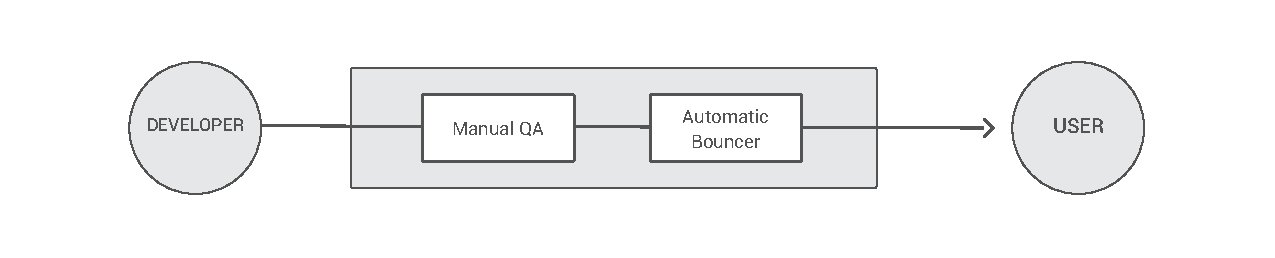
\includegraphics[width=\textwidth]{diagrams/apps_approval_flow.eps}
\caption{App approval in centralized App Stores.}
\label{fig:app_approval_flow}
\end{figure}


By definition, the App Store is a channel between the developer and the user\footnote{This section was contributed by Joao Carneiro, Aptoide backend team member}.

% include contribution from João Carneiro
In order to enforce security, legal and business requirements, App Stores define limits in terms of acceptable app behaviour and/or content. These policies also mirror the store's philosophy (e.g. defining the acceptable content) and protect both users and developers against unwanted or potentially dangerous behaviour thus promoting trust. Policies can include general categories such as safety - protecting against malware behaviour, offensive content or physical harm - or legal - protecting privacy and intellectual property. More restrictive stores such as the Apple App Store also imposes strict rules regarding the user interface design, minimum functionality and quality. \cite{GooglePolicyWebsite} \cite{ApplePolicyWebsite}

%XXX I don't get the meaning of "general categories"

The risk of infringement occurs when new apps are added to the store. Therefore stores which are open to public upload of apps (e.g. Google Play Store or Apple Play Store allow submission by developers) need to ensure that uploaded apps abide by their rules by putting them through a reviewing process. The app approval flow is a critical process for App Stores as it ensures the compliance of new apps to the store's policy.

The app screening may be performed through manual and/or automatic processes and differ between stores as they are defined by their own policies. The manual process involves a group of people (typically belonging to the Quality Assurance and/or the Security Team) who manually install and test apps on real devices. They examine the apps' behaviour and content in order to decide whether each app respects the store's policy. The automatic process consists of a computer program which automatically analyses the submitted apps and compares features to a given dataset of rules, signatures, unwanted apps, content or behaviour. Multiple techniques may be used by the program to automatically classify given apps into unwanted, accepted or unknown states\cite{Bhattacharya2017}.

Google's Play Store and Apple's App Store, the current largest and most well-known app stores use a combination of both processes. When a new app is submitted to their store they first go through an automatic process which will automatically discard identified unwanted apps and then proceed to the manual process. However, the two stores differ in the techniques they use in their automatic processes and the amount of apps that go through manual reviewing\cite{AppleInsiderWebsite}\cite{AndroidWhitePaper}.

Apple App Store approval flow is simple. All submitted apps go through an automatic static analysis process, a method which examines the app code without running it. In this process, the apps are analysed for traces of calls to the Apple's private API as the company's policy only allows calls to their public API. The identified apps are discarded while all the remaining apps are passed on for manual reviewing \cite{AppleInsiderWebsite}\cite{AppleApprovalFortune}. Apple states the following most common reasons for failing their strict manual reviewing process: crashes and bugs, broken links, placeholder content, incomplete information, inaccurate description, misleading users, substandard user interface, advertisements, web clipping, similar apps and not enough lasting value \cite{AppleReviewRejections}. According to apple, the complete review process takes on average between 24 (50\%) to 48 hours (90\% of submitted apps)\cite{AppleReviewTime}. 

Google's Play Store has more evolved reviewing system where the automatic process involves a complex machine learning engine. This engine relies on multiple technologies including static and dynamic analysis (where both code and runtime behaviour is analysed), heuristic and similarity analysis (for finding new trends of unwanted apps) and signatures (identifying known unwanted apps). The engine also includes features from external independent security research as well as the developer's behaviour (history with other apps and billing profile) as well as meta-data such as ratings and downloads. The automatic process assigns to each application a risk level ranging from safe to harmful. Low risk applications are automatically accepted and high risk applications ae automatically rejected. Apps with medium risk level are submitted for manual reviewing\cite{AndroidWhitePaper}. According to publicly available information Play Store's reviewing process takes on average between 45minutes and 2 hours\cite{AndroidReviewTime}.

Although these app approving systems are capable of detecting a large number of unwanted apps they also pose problems to developers. Apple's automatic process has shown problems with false positives and rejecting legitimate apps \cite{AppleInsiderWebsite} and their strict policy is known to frequently changing the categories of rejected apps posing problems to developers of such apps. Also, Apple's reviewing process strongly based on human analysis is known to have flaws, namely not being able to detect apps which hide their malware behaviour being inactive for a given amount of time and showing a regular behaviour in order to escape the human test\cite{AppleFlaws1}. Other reports \cite{AppleFlaws2} have also shown a big presence of scamware in Apple's store where apps are able to scam users into paying for unneeded services. Google's more automated system has also been shown to have flaws \cite{AppleApprovalFortune} due to its more permissive system with apps being accepted without manual evaluation. Frequent security reports show breaches in the security control of Play Store reporting the existence of multiple malware (ransomware, backdoor, trojans) infected apps compromising several millions of devices and thus posing serious threats to users \cite{GoogleMalware1}\cite{GoogleMalware2}\cite{GoogleMalware3}.

\medskip

Both Apple's App Store and Google's Play Store have a history of refusing and banning apps. Examples of recent complaints include the rejection of the social network GAB's app by both Apple and Google\cite{AppRefusedGAB}, the refusal of music streaming Spotify app update\cite{AppleRefuseSpotify} or the Anti-Spam App\cite{AppleRefuseTRIAD} by Apple and the rejection of Popcorn Time, TubeMate, Adguard or Fildo by Google. \cite{GoogleBannedApps}. These rejections are however often considered unfair by developers who claim an abusive and anticompetitive behaviour as the apps conflict with other services provided by the app stores and have motivated complaints to legal authorities\cite{AntiCompetitiveClaim}.

\medskip

As described above, several risks can be found from the current centralized app approval processes:

\begin{tcolorbox}[enhanced jigsaw,sharp corners, drop fuzzy shadow=ShadowColor]

The {\bf\em R3.1: Risk of Malware} is the possibility of an app or game submitted to the app store being infected with a virus or a malware that steal data or damages the user device.

The {\bf\em R3.2: Risk of user data leak} consists in the information regarding the user being leaked to third-parties for advertising purposes. Information about the user preferences is aggregated in DMP platforms and later used by advertising in programmatic / RTB targeting.

%XXX again, R3.2 is just a copy and paste of R1.4

The {\bf\em R3.3: Risk of censorship} when an app store blocks the publishing of an app or game based in political, religious or social factors that are subjective and totally unrelated with technical aspects. The censorship can be self-inflicted when the company running the app store follows orders or guidelines of national governments or can be result of technical external restrictions that limits the access to the app store (great firewall of China, for example).

The {\bf\em R3.4: Risk of arbitrary decisions} happens when the app store denies the distribution of an app based in ``anti-competition claused''\cite{PlayTermsService} or other reasons only related of its business interest, even if the interest is in other markets or industries.

\end{tcolorbox}

\subsection{Paper organization}

This paper is organized in the following chapters. In this chapter we started to introduce the flows, the current challenges and the flaws they carry.

Chapter \ref{sec:design} will propose the overall design of the solution for the core app store flows supported by blockchain technology. 

Chapter \ref{sec:protocol} will deep dive in the blockchain technology, presenting the main data structures and algorithms that are proposed.

The current limitations of the blockchain technology when applied to app stores are introduced in chapter \ref{sec:limitations}.

In chapter \ref{sec:related}, related work that shares common approaches with App Coins protocol are introduced, as well as projects that inspired parts of the App Coins protocol.

% TODO replacing 6 by the \ref tag

The future protocol developments will be included in chapter 6 and this document will end with acknowledging the contributions of the several community members that contributed to this document with their suggestions and opinion.


